\documentclass[a4paper,
fontsize=11pt,
%headings=small,
oneside,
numbers=noperiodatend,
parskip=half-,
bibliography=totoc,
final
]{scrartcl}

\usepackage[babel]{csquotes}
\usepackage{synttree}
\usepackage{graphicx}
\setkeys{Gin}{width=.4\textwidth} %default pics size

\graphicspath{{./plots/}}
\usepackage[ngerman]{babel}
\usepackage[T1]{fontenc}
%\usepackage{amsmath}
\usepackage[utf8x]{inputenc}
\usepackage [hyphens]{url}
\usepackage{booktabs} 
\usepackage[left=2.4cm,right=2.4cm,top=2.3cm,bottom=2cm,includeheadfoot]{geometry}
\usepackage{eurosym}
\usepackage{multirow}
\usepackage[ngerman]{varioref}
\setcapindent{1em}
\renewcommand{\labelitemi}{--}
\usepackage{paralist}
\usepackage{pdfpages}
\usepackage{lscape}
\usepackage{float}
\usepackage{acronym}
\usepackage{eurosym}
\usepackage{longtable,lscape}
\usepackage{mathpazo}
\usepackage[normalem]{ulem} %emphasize weiterhin kursiv
\usepackage[flushmargin,ragged]{footmisc} % left align footnote
\usepackage{ccicons} 
\setcapindent{0pt} % no indentation in captions

%%%% fancy LIBREAS URL color 
\usepackage{xcolor}
\definecolor{libreas}{RGB}{112,0,0}

\usepackage{listings}

\urlstyle{same}  % don't use monospace font for urls

\usepackage[fleqn]{amsmath}

%adjust fontsize for part

\usepackage{sectsty}
\partfont{\large}

%Das BibTeX-Zeichen mit \BibTeX setzen:
\def\symbol#1{\char #1\relax}
\def\bsl{{\tt\symbol{'134}}}
\def\BibTeX{{\rm B\kern-.05em{\sc i\kern-.025em b}\kern-.08em
    T\kern-.1667em\lower.7ex\hbox{E}\kern-.125emX}}

\usepackage{fancyhdr}
\fancyhf{}
\pagestyle{fancyplain}
\fancyhead[R]{\thepage}

% make sure bookmarks are created eventough sections are not numbered!
% uncommend if sections are numbered (bookmarks created by default)
\makeatletter
\renewcommand\@seccntformat[1]{}
\makeatother

% typo setup
\clubpenalty = 10000
\widowpenalty = 10000
\displaywidowpenalty = 10000

\usepackage{hyperxmp}
\usepackage[colorlinks, linkcolor=black,citecolor=black, urlcolor=libreas,
breaklinks= true,bookmarks=true,bookmarksopen=true]{hyperref}
\usepackage{breakurl}

%meta
%meta

\fancyhead[L]{B. Kaden\\ %author
LIBREAS. Library Ideas, 38 (2020). % journal, issue, volume.
\href{http://nbn-resolving.de/}
{}} % urn 
% recommended use
%\href{http://nbn-resolving.de/}{\color{black}{urn:nbn:de...}}
\fancyhead[R]{\thepage} %page number
\fancyfoot[L] {\ccLogo \ccAttribution\ \href{https://creativecommons.org/licenses/by/4.0/}{\color{black}Creative Commons BY 4.0}}  %licence
\fancyfoot[R] {ISSN: 1860-7950}

\title{\LARGE{Kolumne Bibliotheksphilokartie \#1: Die McLaughlin Public Library in Oshawa}}% title
\author{Ben Kaden} % author

\setcounter{page}{1}

\hypersetup{%
      pdftitle={Kolumne Bibliotheksphilokartie \#1: Die McLaughlin Public Library in Oshawa},
      pdfauthor={Ben Kaden},
      pdfcopyright={CC BY 4.0 International},
      pdfsubject={LIBREAS. Library Ideas, 38 (2020).},
      pdfkeywords={Bibliothek, Postkarte, Philokartie},
      pdflicenseurl={https://creativecommons.org/licenses/by/4.0/},
      pdfcontacturl={http://libreas.eu},
      baseurl={http://libreas.eu},
      pdflang={de},
      pdfmetalang={de}
     }



\date{}
\begin{document}

\maketitle
\thispagestyle{fancyplain} 

%abstracts
\begin{abstract}
\noindent
In einer neuen Kolumne wird Ben Kaden regelmäßig eine Ansichtskarte mit
Bibliotheksbezug aus seiner Sammlung kurz vorstellen.
\end{abstract}

%body
Kanada liegt im Covid-Jahr 2020, das die Reiseoptionen aus Berliner
Sicht auf einen Ausflug ins Land Brandenburg zusammenschrumpfen ließ, in
noch weiterer Ferne als sonst. Und selbst wenn man fahren würde, wäre
ein Ausflug nach Oshawa vielleicht nicht die erste Adresse,
möglicherweise aber die zweite, denn von Toronto ist es gar nicht so
weit. Da wir aber ohnehin weitgehend nur in der Vorstellung verreisen
und diese Vorstellung an, zum Beispiel, eine Ansichtskarte zurückbinden,
brauchen wir diesen Umweg gar nicht. Direkt neben dem Rathaus der
kleinen Großstadt und zugleich kanadischen Automobilmetropole und nur
einen Steinwurf entfernt vom Oshawa Creek, an dessen Ufer ein Rad- und
Wanderweg direkt zum Lake Ontario führt, liegt die McLaughlin Branch der
Oshawa Public Library. Gestiftet wurde sie vom Automobil-Unternehmer und
Großspender Samuel McLaughlin, der sich zumindest in diesem Fall in der
Tradition Andrew Carnegies bewegte und dies auch deshalb, weil seine
Filiale 1954 die 1906 vom Carnegie Fund finanzierte und für die
Bedürfnisse der damaligen Gegenwart viel zu beengte Zweigstelle der
Stadt ablöste. McLaughlin, reichster und prominentester Einwohner der
Stadt, half damit auch dem damaligen Bürgermeister Mike Starr aus einer
verfahrenen Situation. Diesem gelang es nämlich nicht, den Bau einer
neuen städtischen Bibliothek durchzusetzen. Eine kommunale
Versorgungslücke, die auch McLaughlin auffiel. Er rief daher irgendwann
im Frühsommer 1952 direkt bei Mike Starr durch und bot an, das Gebäude
zu stiften, wenn die Stadt das Land bereitstellte. Danach ging alles
sehr schnell. Am 22. Juli 1952 konnte die Lokalzeitung Daily
Times-Gazette auch auf der Titelseite vermelden: \enquote{Modern library
will have all facilities}. Als Architekt wurde der 1897 geborene Arthur
Hunter Eadie verpflichtet, der bereits 1947 das Mausoleum für Samuel
McLaughlin geplant hatte, wobei vermutlich weder er noch der 1871
geborene McLaughlin selbst davon ausgingen, dass dieser über 100 Jahre
alt werden sollte.

Für Arthur Eadie wurde die Bibliothek in Oshawa dagegen ein frühes
Spätwerk. Er starb schon 1956. Die Grundsteinlegung für die Bibliothek
erfolgte im November 1953. Die Architektursprache orientiert sich am
sogenanneten Prairie Style, wie man ihn von den Häusern Frank Lloyd
Wrights kennt. Naturverbunden, klar gegliedert, die Horizontale
betonend, das Handwerk zeigend und zugleich genuin nordamerikanisch --
Wright nannte es \enquote{married to the ground} und Eadie fand eine
entsprechende Interpretation, auch wenn das Bibliotheksgebäude seiner
Funktion gemäß am Ende ein eher molliger Block wurde als ein elegantes
Prairie House Wright'schen Zuschnitts. Am 2. Dezember 1954 erfolgte die
offizielle Eröffnung des McLaughlin-Gebäudes durch den damaligen
Premierminister von Ontario, Leslie Frost, und Samuel McLaughlin, was
der Branche des Spenders gemäß auch mit einem großen Artikel in der
Zeitschrift \enquote{Canadian Motorist} gewürdigt wurde und zu einer
Spezialsammlung an Gebrauchsanleitungen für Automobile im Bestand der
Bibliothek führte. Selbiger wurde immerhin bis 2004 von General Motors
regelmäßig erweitert. Im Haus gab es eine Reihe von großformatigen
Wandbildern, unter anderem von der Künstlerin und Tochter des Stifters,
Isabel McLaughlin, sowie William Winter.

Die kleine und nun offenbar überflüssige Carnegie-Filiale in Oshawa
wurde im Januar 1957 abgerissen, ein Schicksal, das sie mit mindestens
14 weiteren der insgesamt 111 Carnegie-Biblio\-the\-ken in Ontario teilte.

\begin{figure}[ht!]
\centering
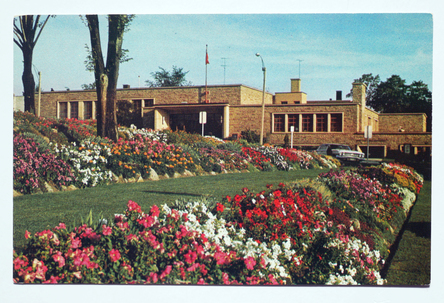
\includegraphics[width=0.9\columnwidth]{img/oshawa-public-library.jpg}
\caption{Ansichtskarte McLaughlin Public Library in Oshawa}
\end{figure}

Aus Sicht der Bibliotheks-Philokartie ist die Ausgabe des in Vancouver
beheimateten Ansichts\-karten-Imprints Traveltime Products nicht unbedingt
selten. Es ist zugleich die einzige Ansicht zu dieser Bibliothek, die
mir bisher begegnete. Die Firma produzierte ihr Kartensortiment in den
1960er und 1970er Jahren, was sichtbar zur Anmutung des Bilds passt. An
der Komposition fällt vor allem auf, wie zurückhaltend, ja fast
versteckt die Bibliothek über die Zierbeete, fast Zierhügel von der
Queen Street aus fotografiert wurde. Zum Prärie-Stil der Architektur
passt das vielleicht weniger, wohl aber zum kanadischen Understatement.
Das Gebäude wird nicht bombastisch inszeniert, sondern fügt sich
harmonisch in die Stadtlandschaft. Eines dieser Autos, die man früher
Straßenkreuzer nannte, parkt etwas schief im Bild, lärmt aber weder
visuell noch sonst irgendwie störend herum. Es herrscht Ruhe am Oshawa
Creek. Blumen dominieren und eigentlich ist es so vielmehr eine Aufnahme
der öffentlichen Gartenbaukultur von Oshawa denn eine der Bibliothek. So
würde die Legende der Karte -- \enquote{McLaughlin Public Library with a
beautiful flower garden in the foreground} -- durchaus auch invertiert
passen: \enquote{A beautiful flower garden with the McLaughlin Public
Library in the background}. So oder so bleibt es natürlich eine
reizvolle Bibliotheksansichtskarte von einem, von Berlin aus gesehen,
aktuell denkbar fernen Ort.

%autor
\begin{center}\rule{0.5\linewidth}{0.5pt}\end{center}

\textbf{Ben Kaden} ist Mitherausgeber von LIBREAS und beschäftigt sich
abseits seiner bibliothekswissenschaftlichen Aktivitäten zunehmend mit
dem Themenfeld der ``Philokartie''. Zuletzt erschien von ihm zum Thema
die Publikation ``Karten zur Ostmoderne'' (Leipzig: sphere, 2020). Eine
fortlaufende Sammlungsdokumentation gibt es unter
\url{https://benkaden.tumblr.com/}.

\end{document}
